\PassOptionsToPackage{table,usenames,dvipsnames,x11names}{xcolor}
\documentclass[english,serif,mathserif]{beamer}
\usetheme[informal]{gc3}

\usepackage[T1]{fontenc}
\usepackage[utf8]{inputenc}
\usepackage{babel}

\usepackage{gc3}

\usepackage{colortbl}
\makeatletter
\rowcolors{1}{uzh@blue!10}{white}
\makeatother

\usepackage{dcolumn}
\newcolumntype{d}[1]{D{.}{\cdot}{#1} }


\begin{document}

%% Optional Argument in [Brackets]: Short Title for Footline
\title[Spark]{An Insufficient Introduction to Spark}
\subtitle{Part 0: Introduction to this Training}
\author{Riccardo Murri \texttt{<riccardo.murri@gmail.com>}}
\date{2019-02-11}

%% Makes the title slide
\maketitle


\begin{frame}
  \begin{center}
    {\Huge Welcome!}
  \end{center}
\end{frame}


\begin{frame}
  \frametitle{Prerequisites}
  This course assumes some experience with Python programming.

  \+
  I try to recall what is needed for exercises, but you will need
  to be able to write a function on your own and not to be puzzled
  about lists and tuples, or methods and function calls.
\end{frame}


\begin{frame}
  \frametitle{Course outline}
  \begin{enumerate}
  % \item What is Spark?
  \item The Map/Reduce programming model
  \item RDDs
  \item DataFrames and SQL
  \item Window Functions
  \end{enumerate}
\end{frame}


\begin{frame}
  \frametitle{Next steps}

  The course will be structured as a mixture of slides and hands-on
  sessions for practicing PySpark programming.

  \+
  So, the very first step is making sure you can access the Jupyter/IPython
  server for running the exercise notebooks.
\end{frame}


\part{How to run Python code}

\begin{frame}
  \frametitle{The IPython notebook, I}

  \begin{columns}[t]
    \begin{column}{0.5\textwidth}
      \begin{center}
        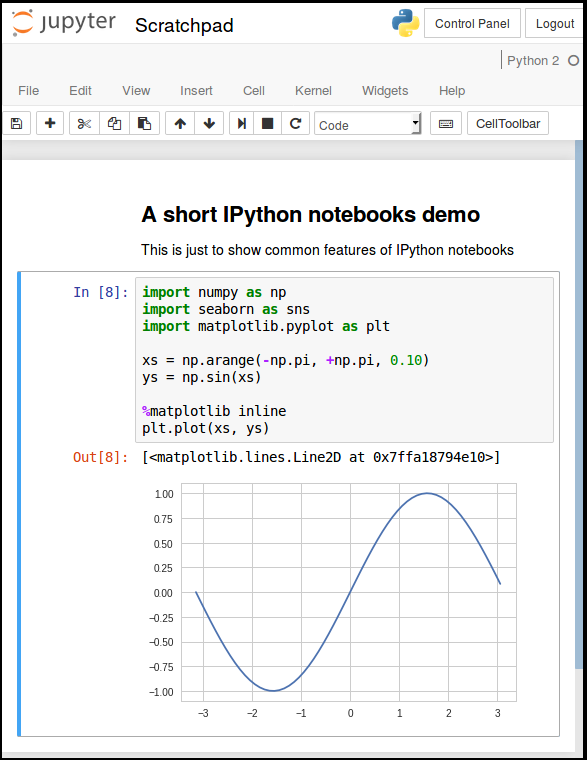
\includegraphics[width=1.00\linewidth]{fig/nb.png}
      \end{center}
    \end{column}
    \begin{column}{0.5\textwidth}
      \small

      An appealing way of interacting with Python
      is through \emph{IPython notebooks}.

      \+
      Notebooks are made of ``cells'', which come in two flavors:
      \begin{itemize}
      \item documentation cells, containing text formatted according to the
        \href{http://commonmark.org/help/}{Markdown} conventions;
      \item code cells, containing arbitrary Python code
      \end{itemize}
    \end{column}
  \end{columns}
\end{frame}


\begin{frame}
  \frametitle{The IPython notebook, II}

  To run Python code in the notebook:
  \begin{itemize}
  \item Type your code in a cell besides the {\ttfamily\bfseries\color{blue}
      In~[~]:} (multiple lines are allowed)
  \item Press \textbf{Ctrl+Enter} to evaluate the cell (prompt changes to
    {\ttfamily\bfseries\color{blue} In~[*]:}) --- or press \textbf{Alt+Enter} to
    evaluate the code \emph{and} open a new code cell.
  \item When the Python kernel has done computing, the result appears \emph{under} the
    code cell marked with a {\ttfamily\bfseries\color{red} Out~[~]:} label.
  \end{itemize}

\end{frame}


\end{document}


%%% Local Variables:
%%% mode: latex
%%% TeX-master: t
%%% End:
